\chapter{Conclusiones}
\label{chp:conclusiones}

% \section{Introducción}

% Durante la fase experimental, el seguimiento de la evolución del sistema multifásico Aceite-Salmuera-Surfactante por medios reológicos cuantitativos y análisis de imágenes, nos dieron la evidencia suficiente para plantear la formación de una nueva fase llamada organogel, a continuación se presenta el mecanismo de formación de dicha fase propuesto.

% \section{Proceso de emulsificación en presencia de tensoactivos}
% El agua congénita y el aceite son inmiscibles, al ser sometidos a una agitación debida a un esfuerzo mecánico, las dos fases se mezclan formando una emulsión inestable, que una vez en reposo, se segrega regresando nuevamente a las dos fases originales. Este proceso se muestra en la \autoref{fig:conclu1}.

% \begin{figure}[h]
%     \centering
%     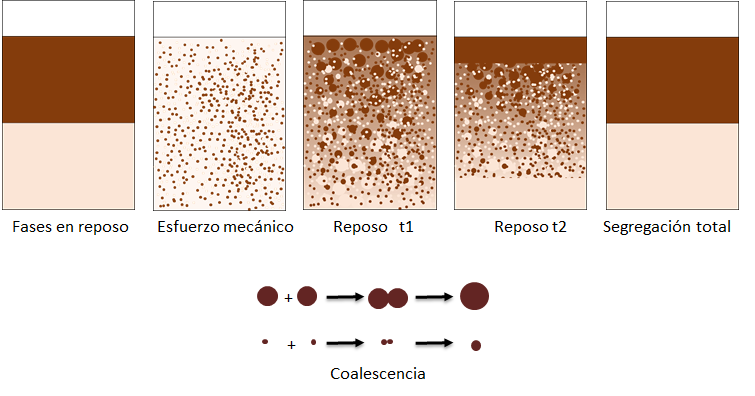
\includegraphics[width = \textwidth]{Graphics/Conclutions/coales_1.png}
%     \caption[Proceso de emulsificación sin tensoactivos]{Proceso de emulsificación sin presencia de tensoactivos sistema Aceite-Agua.}
%     \label{fig:conclu1}
% \end{figure}


% En presencia del producto (\emph{Amesus $3100$ y $3200$}), el aceite disperso coalesce, mientras que la parte acuosa forma gotas rodeadas por los activos del producto, que, al tener un tamaño por arriba de un diámetro crítico coalescen y por debajo del mismo forman gotas estables que dan origen a la microemulsión. Cuando estas gotas se aglutinan sus interfases forman una red y se genera el hidrogel \autoref{fig:conclu2}. Esta red se confirmó de manera visual con el análisis de imágenes, presentado en el \autoref{chp:resultados}.

% \begin{figure}[h]
%     \centering
%     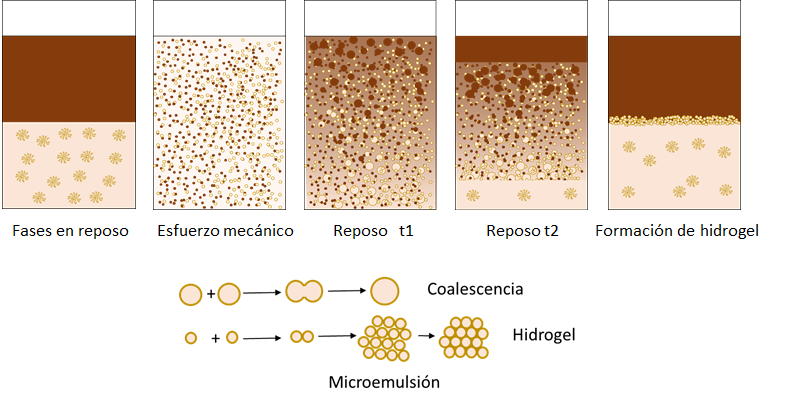
\includegraphics[width=\textwidth]{Graphics/Conclutions/coales_2.png}
%     \caption[Proceso de emulsificación sin tensoactivos]{Proceso de emulsificación en presencia de tensoactivos: sistema Aceite-Salmuera-Surfactante.}
%     \label{fig:conclu2}
% \end{figure}

% En presencia de aceite, el hidrogel se hincha elongando las gotas de agua que se fracturan generando a una red que recubre gotas de aceite y dando origen al organogel. Las gotas de aceite siguen hinchándose hasta que la red se rompe y se drena el producto junto con le agua congénita a la fase acuosa.

% \begin{figure}[h]
%     \centering
%     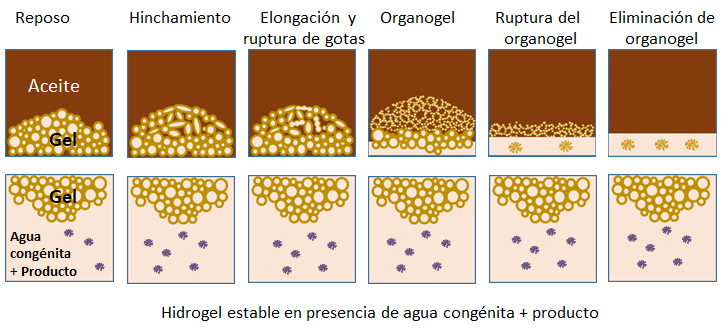
\includegraphics[width=\textwidth]{Graphics/Conclutions/coales_3.png}
%     \caption[Proceso de emulsificación sin tensoactivos]{Proceso de formación de la fase organogel: sistema Aceite-Salmuera-Surfactante.}
%     \label{fig:conclu3}
% \end{figure}


El seguimiento de la evolución del sistema Aceite-Salmuera-Surfactante resumido en la presente sección, es evidencia suficiente para confirmar la presencia de un material estructurado con propiedades viscoelásticas que varían con el tiempo de convivencia entre las fases, la concentración de surfactante, condiciones de temperatura y salinidad en el sistema.

\subsubsection{Evolución del drenado y análisis de imágenes}
El seguimiento del drenado de las fases y el análisis de imágenes, confirman la presencia de estructura dentro del fluido similar a la descrita por (\cite{Nishinari2009}) como un fluido estructurado o gel. 

\subsubsection{Tensión interfacial}
De manera complementaria el comportamiento de la tensión interfacial permitió determinar experimentalmente la concentración miscelar crítica del sistema lo que deriva en proponer un mecanismo válido para la formación de la fase organogel a partir del sistema Aceite-Salmuera-Surfactante.

\subsubsection{Caracterización reológica}
Las pruebas reológicas realizadas muestran la existencia de un punto de cedencia en el reograma de la fase para diferentes condiciones de concentración y temperatura lo que confirma las propiedades viscoelásticas del material que además son dependientes del tiempo de deformación según se confirmó durante las pruebas de tiempo de reestructuración.

\subsubsection{Trabajo posterior}
La capacidad del nueva fase organogel, presenta características que pueden a aprovecharse para el control de agua y como inhibidor de la corrosión en pozos de aceite de alta temperatura y alta salinidad. 

 Dichas características fueron propuestas y han sido detalladas por el IMP (\cite{WETFOAM}), quedando su estudio fuera del alcance del presente trabajo.
%  donde se llevo a cabo la primer prueba tecnológica en el campo Teotleco donde se aplicó la tecnología.
% IMP-WETFOAM\textsuperscript{\sffamily\textregistered} a través del producto $IMP-AMESUS 3100$ (\cite{WETFOAM}).

El análisis sistematico descrito en el \autoref{chp:metodologia} de este trabajo fué adaptado por los investigadores del IMP, bajo la premisa de que la evidencia encontrada durante la fase experimental (\autoref{chp:resultados}) es contundente y establece un mecanismo válido para la obtención de un organogel a partir de un sistema Aceite-Salmuera-Surfactante.

Los Resultados de la interacción fluido-fluido, y pruebas de desplazamiento en núcleos naturalmente fracturados representativos del campo Teotleco, confirmaron la capacidad de la fase organogel de actuar como barrera selectiva permeable a la fase orgánica (aceite) y capaz de generar canales preferenciales de flujo, reduciendo así la movilidad de agua congénita en el medio fracturado sin afectar la movilidad del aceite (\cite{Elizabeth}).

En 2018 el IMP realizará una segunda prueba tecnológica con en el campo Teotleco utilizando la ya consolidada, plataforma tecnológica IMP-WETFOAM, aprovechando las características de una fase organogel dentro de un yacimiento en condiciones similares de temperatura, salinidad y fluidos contenidos.

Este trabajo contribuyo de lo que posteriormente se coloca en la industria como una alternativa comercial para la recuperación adicional de aceite en yacimientos naturalmente fracturados y en condiciones de alta salinidad y temperatura.